\documentclass{article}

\usepackage[utf8]{inputenc}
\usepackage{graphicx}
\usepackage[english,dutch]{babel}

\author{Thom Wiggers\\ s4119444}
\title{Informatiesystemen 1}

\begin{document}
\maketitle
\tableofcontents
\section{Huishoudelijke mededelingen}
Dit project maak ik individueel. 

\section{Taak 1 - ORC}
\subsection{Inleiding}
\label{sub:1-orm-inleiding}
ORM is een methode om door middel van modellen systemen te ontwikkelen waarbij
gepoogd wordt zo min mogelijk fouten toe te laten en zo veel mogelijk
redundantie in de opgeslagen gegevens te voorkomen. 

ORM bestaat voornamelijk uit een verzameling afspraken over taalgebruik en
notaties. Hierdoor zou een goed model ook voor niet-domeinexperts leesbaar
en begrijpbaar moeten zijn. 

Hoewel ORM modellen vooral worden omgezet naar klassieke relationele
(SQL)-databases, is het ook mogelijk om direct 'vragen` te stellen aan
een dataset in ORM. Deze querytaal staat bekend als Object-Role Calculus 
(ORC).

Ik ga hier proberen ORC te vergelijken met de SQL taal, door middel van het
vergelijken van enkele verschillende queries, zoekvragen, waarbij ik ook 
in ga op de fundamentele verschillen tussen de twee verschillende systemen.
Hiervoor zal ik een voorbeeldsysteem beschrijven, zowel uitgevoerd in ORM 
als draaiende op de populaire relationele database postgreSQL.

\subsection{Systeem}
Ik ga hier een voorbeeldsysteem beschrijven van een webwinkel waar men 
schoenen verkoopt. In deze webwinkel houdt men bestellingen bij, en 
profielen van klanten. Bestellingen kunnen bestaan uit een of meerdere
paren schoenen, in verschillende maten en aantallen.

\subsubsection{ORM}
\begin{figure}[htp]
  \centering
  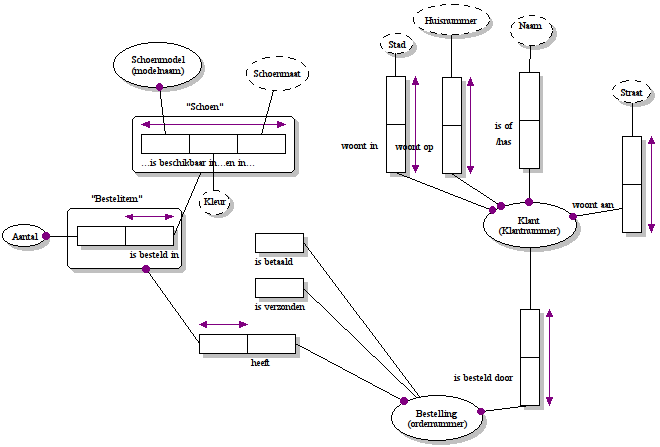
\includegraphics[keepaspectratio=true, width=345pt]{model1.png}
  \caption{ORM Model van het voorbeeldsysteem
    \caption{ORM Model van het voorbeeldsysteem}
  \label{img:model1}
\end{figure}

\Large{--- Check syntax --- }

\begin{verbatim}
Schoen: Schoenmodel (modelnaam) is beschikbaar
    in Schoenmaat en is beschikbaar in Kleur.
Bestelitem: Schoen is besteld in aantal.
Bestelling (ordernummer) heeft Bestelitem.
Bestelling (ordernummer) is besteld door 
   Klant (klantnummer).
Bestelling is betaald.
Bestelling is verzonden.
Klant (klantnummer) woont aan 
   Straat (straatnaam).
Klant (klantnummer) woont op 
   Huisnummer (nr).
Klant (klantnummer) woont in Stad (naam).
\end{verbatim}

\subsubsection{SQL Tables}


\end{document}
